\begin{figure}[t]
\centering
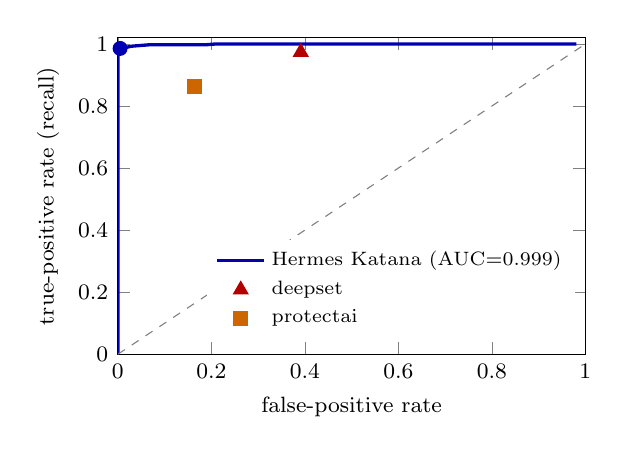
\begin{tikzpicture}
\begin{axis}[
  width=0.62\linewidth, height=5.6cm,
  xlabel={false-positive rate}, ylabel={true-positive rate (recall)},
  xmin=0,xmax=1,ymin=0,ymax=1.02, label style={font=\footnotesize}, tick label style={font=\footnotesize},
  legend style={at={(0.98,0.05)},anchor=south east,font=\scriptsize,draw=none},
  legend cell align=left,
]
\addplot[blue!70!black,very thick,mark=none] coordinates {(0.0000,0.0000) (0.0000,0.0118) (0.0000,0.0237) (0.0000,0.0355) (0.0000,0.0474) (0.0000,0.0592) (0.0000,0.0711) (0.0000,0.0829) (0.0000,0.0948) (0.0000,0.1066) (0.0000,0.1185) (0.0000,0.1303) (0.0000,0.1422) (0.0000,0.1540) (0.0000,0.1659) (0.0000,0.1777) (0.0000,0.1896) (0.0000,0.2014) (0.0000,0.2133) (0.0000,0.2251) (0.0000,0.2370) (0.0000,0.2488) (0.0000,0.2607) (0.0000,0.2725) (0.0000,0.2844) (0.0000,0.2962) (0.0000,0.3081) (0.0000,0.3199) (0.0000,0.3318) (0.0000,0.3436) (0.0000,0.3555) (0.0000,0.3673) (0.0000,0.3791) (0.0000,0.3910) (0.0000,0.4028) (0.0000,0.4147) (0.0000,0.4265) (0.0000,0.4384) (0.0000,0.4502) (0.0000,0.4621) (0.0000,0.4739) (0.0000,0.4858) (0.0000,0.4976) (0.0000,0.5095) (0.0000,0.5213) (0.0000,0.5332) (0.0000,0.5450) (0.0000,0.5569) (0.0000,0.5687) (0.0000,0.5806) (0.0000,0.5924) (0.0000,0.6043) (0.0000,0.6161) (0.0000,0.6280) (0.0000,0.6398) (0.0000,0.6517) (0.0000,0.6635) (0.0000,0.6754) (0.0000,0.6872) (0.0000,0.6991) (0.0000,0.7109) (0.0000,0.7227) (0.0000,0.7346) (0.0000,0.7464) (0.0000,0.7583) (0.0000,0.7701) (0.0000,0.7820) (0.0000,0.7938) (0.0000,0.8057) (0.0000,0.8175) (0.0000,0.8294) (0.0000,0.8412) (0.0000,0.8531) (0.0000,0.8649) (0.0000,0.8768) (0.0000,0.8886) (0.0000,0.9005) (0.0000,0.9123) (0.0000,0.9242) (0.0000,0.9360) (0.0000,0.9479) (0.0000,0.9597) (0.0000,0.9716) (0.0048,0.9810) (0.0145,0.9882) (0.0290,0.9929) (0.0483,0.9953) (0.0676,0.9976) (0.0918,0.9976) (0.1159,0.9976) (0.1401,0.9976) (0.1643,0.9976) (0.1884,0.9976) (0.2077,1.0000) (0.2319,1.0000) (0.2560,1.0000) (0.2802,1.0000) (0.3043,1.0000) (0.3285,1.0000) (0.3527,1.0000) (0.3768,1.0000) (0.4010,1.0000) (0.4251,1.0000) (0.4493,1.0000) (0.4734,1.0000) (0.4976,1.0000) (0.5217,1.0000) (0.5459,1.0000) (0.5700,1.0000) (0.5942,1.0000) (0.6184,1.0000) (0.6425,1.0000) (0.6667,1.0000) (0.6908,1.0000) (0.7150,1.0000) (0.7391,1.0000) (0.7633,1.0000) (0.7874,1.0000) (0.8116,1.0000) (0.8357,1.0000) (0.8599,1.0000) (0.8841,1.0000) (0.9082,1.0000) (0.9324,1.0000) (0.9565,1.0000) (0.9807,1.0000)};
\addlegendentry{Hermes Katana (AUC=0.999)}
\addplot[gray,dashed,mark=none,forget plot] coordinates {(0,0)(1,1)};
\addplot[only marks,mark=*,blue!70!black,mark size=2.5pt,forget plot] coordinates {(0.0048,0.9858)};
\addplot[only marks,mark=triangle*,red!70!black,mark size=3pt] coordinates {(0.3913,0.9739)};
\addlegendentry{deepset}
\addplot[only marks,mark=square*,orange!80!black,mark size=2.5pt] coordinates {(0.1643,0.8626)};
\addlegendentry{protectai}
\end{axis}
\end{tikzpicture}
\caption{ROC of the binary attack/benign decision on \texttt{confirmed\_only\_v2} (AUC 0.999). The filled circle marks Hermes~Katana's deployed operating point (0.48\% FPR, 98.6\% recall); the two public detectors (triangle, square), scored on the same rows, sit at 39.1\% and 16.4\% false-positive rates.}
\label{fig:roc}
\end{figure}
